Controlador utilizando Lógica Paraconsistente Anotada Evidencial $E\tau$



\section{Resultados}

O processo de implementação da LPA2v como parte do núcleo do controlador 
produziu algumas tentativas sendo que segue aquela de melhor resultado, 
não esgotando as formas e tentativas que poderão se seguir 
no decorrer da pesquisa.


%%%%%%%%%%%%%%%%%%%%%%%%%%%%%%%%%%%%%%%%%%%%%%%%%%
%%%%%%%%%%%%%%%%%%%%%%%%%%%%%%%%%%%%%%%%%%%%%%%%%%
%%%%%%%%%%%%%%%%%%%%%%%%%%%%%%%%%%%%%%%%%%%%%%%%%%
%%%%%%%%%%%%%%%%%%%%%%%%%%%%%%%%%%%%%%%%%%%%%%%%%%
\begin{comment}
O código da Figura \ref{fig:codigoGcGct} mostra 
a implementação da função que calcula os graus de Certeza e Contradição 
tendo como parâmetro de entrada dois graus de evidência favoráveis.

A LPA2v foi codificada utilizando variáveis do tipo ponto flutuante 
de forma a trabalhar com os seus parâmetros da mesma forma como a lógica é 
proposta e analisada conceitualmente, por isso, inclusive, 
a utilização de um microcontrolador com um módulo dedicado 
ao cálculo utilizando variáveis desse tipo. 


\begin{figure}[!htb]
\centering
\caption{Código de função que calcula os graus de Certeza e Contradição utilizando LPA2v}
\begin{minipage}{0.9\linewidth}
\begin{lstlisting}
float Gc, Gct;

void LPA2v( float u0, float u1 )
{
  float l0, l1;
  l0 = 1.0 - u0;
  l1 = 1.0 - u1;

  Gc  = u0 - l1;
  Gct = (u0 + l1) - 1.0;
}
\end{lstlisting}
\end{minipage}
\label{fig:codigoGcGct}

{\small Fonte: Próprio autor}
\end{figure}

A função \texttt{LPA2v} possui como parâmetros de entrada 
dois graus de certeza, simplesmente para facilitar o raciocínio,
sendo que os respectivos graus de inceteza 
são declarados como variáveis locais na linha 5 e calculados nas linhas 6 e 7.

As linhas 9 e 10 apresentam o cálculo dos graus de Certeza e Contradição, 
sendo as respectivas variáveis declaradas como globais, linha 1, 
por serem elas utilizadas em outras funções.






\begin{figure}[!htb]
\centering
\caption{Código de função do controlador utilizando a LPA2v}
\begin{minipage}{0.9\linewidth}
\lstset{firstnumber=12}
\begin{lstlisting}
#define KLP 	10
long controlador( long setpoint, long max, long sensor )
{
  float aux, rT, hT;
  long uT;

  rT = (float) setpoint / (float) max;
  hT = (float) sensor   / (float) max;

  if( rT > 1.0 )
    rT = 1.0;
  if( hT > 1.0 )
    hT = 1.0;
  
  aux = (rT * 100.0);

  LPA2v( rT, hT );
  
  uT = (long)(aux + aux * Gct * KLP);
  if( uT > 99 )
    uT = 99;
  if( uT < 0 ) 
    uT = 0;
  return( uT );
}

\end{lstlisting}
\end{minipage}
\label{fig:codigoControladorLPA2v}

{\small Fonte: Próprio autor}
\end{figure}

\end{comment}

%%%%%%%%%%%%%%%%%%%%%%%%%%%%%%%%%%%%%%%%%%%%%%%%%%
%%%%%%%%%%%%%%%%%%%%%%%%%%%%%%%%%%%%%%%%%%%%%%%%%%
%%%%%%%%%%%%%%%%%%%%%%%%%%%%%%%%%%%%%%%%%%%%%%%%%%
%%%%%%%%%%%%%%%%%%%%%%%%%%%%%%%%%%%%%%%%%%%%%%%%%%

A Figura \ref{fig:diagramaBlocosLPA2v} mostra 
o diagrama de blocos da implementação da 
LPA2v inserida na malha de controle. 

\begin{figure}[!h]
\centering
\caption{Diagrama de blocos do controle utilizando a LPA2v}
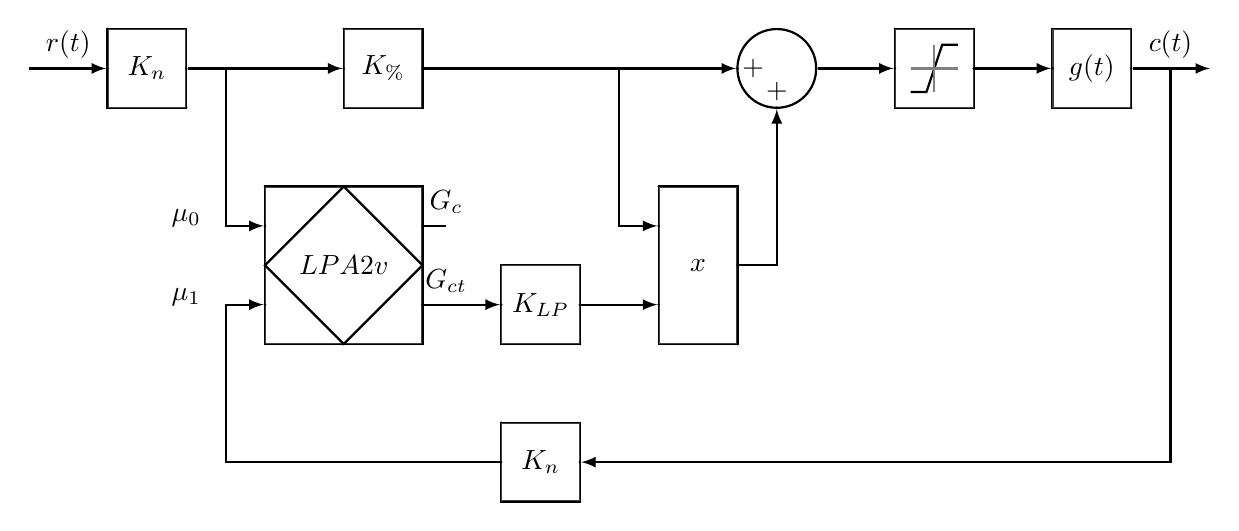
\begin{tikzpicture}[scale=1.0]
\tikzset{ >=latex, inner sep=0pt, outer sep=0pt,  }

%\draw [lightgray, dashed](0,0) grid (15,7);

%%% Blocos 

% K normalização rps -> 0..1
\node [fill=black, circle] (KSP0) at (1,6.5) { };
\node [fill=black, circle] (KSP1) at (2,5.5) { };
\draw[thick] (KSP0) rectangle (KSP1);
\fill[white, nearly transparent] (KSP0) rectangle (KSP1);
\node [fill=black, circle] (KSPin)  at (1.0,6.0) { }; 
\node [fill=black, circle] (KSPout) at (2.0,6.0) { }; 
\node (Kn1) at (1.5,6.0) {$K_n$};

% K normalização  0..1 --> %PWM
\node [fill=black, circle] (KPWM0) at (4,6.5) { };
\node [fill=black, circle] (KPWM1) at (5,5.5) { };
\draw[thick] (KPWM0) rectangle (KPWM1);
\fill[white, nearly transparent] (KPWM0) rectangle (KPWM1);
\node [fill=black, circle] (KPWMin)  at (4.0,6.0) { };
\node [fill=black, circle] (KPWMout) at (5.0,6.0) { };
\node (K100) at (4.5,6.0) {$K_{\%}$};

% Planta
\node [fill=black, circle] (GT0) at (13,6.5) { };
\node [fill=black, circle] (GT1) at (14,5.5) { };
\draw[thick] (GT0) rectangle (GT1);
\fill[white, nearly transparent] (GT0) rectangle (GT1);
\node [fill=black, circle] (GTin)  at (13.0,6.0) { };
\node [fill=black, circle] (GTout) at (14.0,6.0) { };
\node (planta) at (13.5,6.0) {$g(t)$};

% Saturação
\node [fill=black, circle] (SAT0) at (11,6.5) { };
\node [fill=black, circle] (SAT1) at (12,5.5) { };
\draw[thick] (SAT0) rectangle (SAT1);
\fill[white, nearly transparent] (SAT0) rectangle (SAT1);
\node [fill=black, circle] (SATin)  at (11.0,6.0) { };
\node [fill=black, circle] (SATout) at (12.0,6.0) { };
\draw [thick] (11.2,5.7) -- (11.4,5.7) -- (11.6,6.3) -- (11.8,6.3);
\draw [gray, thick] (11.2,6.0) -- (11.8,6.0);
\draw [gray, thick] (11.5,5.7) -- (11.5,6.3);

% Multiplicacao
\node [fill=black, circle] (MUL0) at (8,4.5) { };
\node [fill=black, circle] (MUL1) at (9,2.5) { };
\draw[thick] (MUL0) rectangle (MUL1);
\fill[white, nearly transparent] (MUL0) rectangle (MUL1);
\node [fill=black, circle] (MULin0) at (8.0,4.0) { };
\node [fill=black, circle] (MULin1) at (8.0,3.0) { };
\node [fill=black, circle] (MULout) at (9.0,3.5) { };
\node (multi) at (8.5,3.5) {$x$};

% Klp
\node [fill=black, circle] (KLP0) at (6,3.5) { };
\node [fill=black, circle] (KLP1) at (7,2.5) { };
\draw[thick] (KLP0) rectangle (KLP1);
\fill[white, nearly transparent] (KLP0) rectangle (KLP1);
\node [fill=black, circle] (KLPin)  at (6.0,3.0) { };
\node [fill=black, circle] (KLPout) at (7.0,3.0) { };
\node (KLP) at (6.5,3.0) {$K_{LP}$};

% Sensor
\node [fill=black, circle] (KS0) at (6,1.5) { };
\node [fill=black, circle] (KS1) at (7,0.5) { };
\draw[thick] (KS0) rectangle (KS1);
\fill[white, nearly transparent] (KS0) rectangle (KS1);
\node [fill=black, circle] (KSin)  at (7.0,1.0) { };
\node [fill=black, circle] (KSout) at (6.0,1.0) { };
\node (Kn2) at (6.5,1.0) {$K_n$};

% LPA2v
\node [fill=black, circle] (LPA0) at (3,4.5) { };
\node [fill=black, circle] (LPA1) at (5,2.5) { };
\draw[thick] (LPA0) rectangle (LPA1);
\fill[white, nearly transparent] (LPA0) rectangle (LPA1);
\node [fill=black, circle] (LPAu0) at (3.0,4.0) { };
\node [fill=black, circle] (LPAu1) at (3.0,3.0) { };
\node [fill=black, circle] (LPAgc)  at (5.0,4.0) { };
\node [fill=black, circle] (LPAgct) at (5.0,3.0) { };
\draw [thick] (4.0,4.5) -- (5.0,3.5) -- (4.0,2.5) -- (3.0,3.5) -- (4.0,4.5);
\node (LPA2v) at (4.0,3.5) {$LPA2v$};
\draw [thick] (LPAgc) -- (5.3,4.0);
\node (LPA2vu0)  at (2.0,4.1) {$\mu _0$};
\node (LPA2vu1)  at (2.0,3.1) {$\mu _1$};
\node (LPA2vGc)  at (5.3,4.3) {$G_c$};
\node (LPA2vGct) at (5.3,3.3) {$G_{ct}$};


% Somador
\node [fill=black, circle] (SUM) at (9.5,6.0) { };
\filldraw[fill=white,thick] (SUM) circle (5mm);
\node [fill=black, circle] (SUMin0) at ( 9.0,6.0) { };
\node [fill=black, circle] (SUMin1) at ( 9.5,5.5) { };
\node [fill=black, circle] (SUMout) at (10.0,6.0) { };
\node (Sum0) at (9.2,6.0) {$+$};
\node (Sum1) at (9.5,5.7) {$+$};



%%% Linhas 

% set point
\draw [->, thick] (0.0,6.0) -- (KSPin);
\node (rt) at (0.5,6.3) {$r(t)$};

% setpoint -> normalização %PWM
\draw [->, thick] (KSPout) -- (KPWMin);

% normalização %PWM -> SUM
\draw [->, thick] (KPWMout) -- (SUMin0);

% SUM -> Saturação
\draw [->, thick] (SUMout) -- (SATin);

% Saturação -> GT
\draw [->, thick] (SATout) -- (GTin);

% GT -> fim
\draw [->, thick] (GTout) -- (15,6);
\node (ct) at (14.5,6.3) {$c(t)$};

% LPA2v Gct -> KLP
\draw [->, thick] (LPAgct) -- (KLPin);

% KLP -> MULin1
\draw [->, thick] (KLPout) -- (MULin1);

% normalização 0..1 -> LPA2v u0
\draw [->, thick] (2.5,6.0) -- (2.5,4.0) -- (LPAu0);

% normalização %PWM -> MULT in0
\draw [->, thick] (7.5,6.0) -- (7.5,4.0) -- (MULin0);

% MULT out -> SUM in1
\draw [->, thick] (MULout) -- (9.5,3.5) -- (SUMin1);

% Fim -> sensor
\draw [->, thick] (14.5,6.0) -- (14.5,1.0) -- (KSin);

% Sensor -> LPA u2
\draw [->, thick] (KSout) -- (2.5,1.0) -- (2.5,3.0) --(LPAu1);

\end{tikzpicture}
\label{fig:diagramaBlocosLPA2v}

{\vspace{0.2cm} \small Fonte: Próprio autor}
\end{figure}

Temos então a descrição dos blocos :

\begin{itemize}
  \item $K_n$: Bloco de normalização da grandeza de velocidade de giro do motor em rotações por segundo para o intervalo fechado entre 0,0 e 1,0. 
São dois bloco, sendo um para o parâmetro de referência, 
ou \emph{setpoint}, e o outro para o sinal do sensor que efetua a 
leitura diretamente na planta de processo;

  \item $K_{\%}$: Normaliza o valor em um intervalo fechado de 0,0 a 1,0 para um intervalo de 0 a 100 correspondente ao parâmetro do acionamento por PWM;

  \item $LPA2v$: Calcula os graus de Certeza e Contradição 
de acordo com os parâmetros de entrada, 
que são os graus de evidência favorável $\mu _0$ e $\mu _1$ e são
respectivamente referentes ao valor desejado e 
ao valor real lido diretamente na planta;

  \item $K_{LP}$: Coeficiente de ganho proporcional do grau de contradição;

  \item $x$: Bloco multiplicador;

  \item $g(t)$: Planta do sistema;

  \item $Soma$: Bloco somador;

  \item \emph{Saturação}: Bloco limitador, impede o valor do PWM ultrapassar seu valor máximo de 100\%. 
\end{itemize}



Para implementação do controlador foram realizados alguns testes 
para verificar a velocidade máxima que o motor alcança, 
chegando ao valor de 85 rotações por segundo (rps), com isso, 
foi possível ajustar o bloco $K_n$ para $\frac{1}{85}$, 
e sabe-se que o limite máximo para entrada em $r(t)$ é 85 e o mínimo é 0.

O bloco $K_\%$ é apenas um fator multiplicador com valor 100.

O bloco da $LPA2v$ apresenta a seguinte proposição:

\emph{ P: O eixo do motor apresenta rotação igual ao valor de referência.}

Para tal proposição, 
são utilizados dois especialistas: 
$\mu _0$ é o grau de crença que refere-se ao valor desejado, 
e corresponde ao valor teórico para acionamento do PWM;
e $\mu _1$, que é o grau de crença com que o motor 
atinge a velocidade de giro desejada, 
é o valor utilizado como realimentação do sistema.

O bloco LPA2v calcula os graus de descrença das respectivas entradas:

\begin{equation}
\lambda _0 = 1- \mu _0   \hspace{1cm}   \lambda _1 = 1 - \mu_1 
\end{equation}

Para o cálculo dos graus de Certeza e Contradição são utilizados:

\begin{equation}
P _{(\mu_0, \lambda_1)}
\end{equation}


Os resultados da ação de controle utilizando a LPA2v são mostrados na 
Figura \ref{fig:acaoLPA2v}, onde pode-se ver que 
para um $K_{LP}$ variando de 4 até 10, 
o sistema apresenta comportamento que atende aos requisitos de desempenho,
pois o valor de regime entra na janela formada pelo erro de $5\%$ referente
ao valor desejado em um tempo menor do que um $\tau$, ou seja, 2,5s.
Mesmo o sobressinal gerado com $K_{LP} = 10$, 
não chega a ultrapassar o valor limite máximo de erro. 


\begin{figure}[!htb]
\caption{Ação de controle utilizando LPA2v}
\vspace{-1cm}\center\includegraphics[scale=1.6]{./imagens/klpAll.eps}
\label{fig:acaoLPA2v}

{\small Fonte: Próprio autor}
\end{figure}


Em um segundo momento foi gerado um sinal de referência variável,
assumindo valores de patamar diferentes a 
cada intervalo de tempo aproximado de 10s.
A Figura \ref{fig:acaoLPA2vpatam85} mostra 
o sinal de referência junto ao sinal de resposta da planta,
onde nota-se que com um degrau com variação de 25, 
houve um sobressinal, porém para os demais patamares, 
a variação foi menor, e com isso, 
não apresentaram sobressinal. 
Outro ponto notado foi que o erro é cada vez maior quanto maior for o 
valor de desejado, de referência. 



\begin{figure}[!htb]
\caption{Ação de controle utilizando LPA2v para valores alvo variáveis}
\vspace{-1cm}
\center\includegraphics[scale=1.4]{./imagens/patam85.eps}
\label{fig:acaoLPA2vpatam85}

{\small Fonte: Próprio autor}
\end{figure}



Apesar destes detalhes o resultado é tido como muito bom e promissor,
pois possibilitou que a LPA2v fosse testada de forma empírica em um sistema
de controle dinâmico, obtendo uma performance dentro de um padrão mínimo 
estabelecido.





\section{Etapas a serem desenvolvidas}

\begin{itemize}
\item Estudar a LPA2v;
\item Implementar um controlador utilizando LPA2v;
	\begin{itemize}
	\item Estabelecer a configuração do sistema;
	\item Descrever o controlador e parâmetros de ajuste;
	\end{itemize}
\item Otimizar parâmetros e analisar performance;
\end{itemize}


